\def\thedocument{System Requirements Document}
\def\thedate{DATE} % TODO: insert proper date here
\def\theversion{0.1}
\def\thestatus{Working copy}

\documentclass[notitlepage,headsepline,twoside,a4paper,11pt]{report}
\usepackage[english]{babel}
% Uncomment this line if not using XeTeX and you need unicode characters
% \usepackage[utf8]{inputenc}
\usepackage[T1]{fontenc}
\usepackage{listings}
\usepackage{tabularx}
\usepackage[top=2.5cm,bottom=2.5cm,nohead,nofoot]{geometry}
\usepackage{pdfpages}
\usepackage{fancyhdr}
\usepackage{ifthen}
\usepackage{color}
\definecolor{dark-blue}{rgb}{0, 0, 0.6}
\usepackage{hyperref}
\hypersetup{
  pdfpagemode=FullScreen,
  colorlinks=true, 
  linkcolor=dark-blue,
  urlcolor=dark-blue
}

% fulhack för att se till att vi inte får med kapitel-numrering.
\renewcommand{\chaptername}{}
\renewcommand{\thechapter}{}
\renewcommand{\thesection}{\arabic{section}}
\renewcommand{\and}{\\}

\newcommand{\documentstatus}{\small{\theversion\ -- \thestatus}}

\newenvironment{itemize*}{
\begin{itemize}
  \setlength{\itemsep}{1pt}
  \setlength{\parskip}{0pt}
  \setlength{\parsep}{0pt}
}{\end{itemize}}

\def\requirement#1#2{
  \subsubsection*{}
  \noindent
  \setlength{\extrarowheight}{4pt}
  \begin{tabularx}{\linewidth}%
    {l>{\setlength\hsize{0.67\hsize}}X% 
    >{\setlength\hsize{1.33\hsize}}X} 
     \toprule

  % Table content
  \multicolumn{2}{c}{\textbf{#1}} \\ \midrule
  #2
   \bottomrule 
  \end{tabularx} \\ \\ \\
}

\pagestyle{fancy}
\headheight 14pt
\fancyfoot{}
\lhead{\thecode\ \thecourse}
\rhead{\theproject}
\fancyfoot[LE,RO]{\thepage}
\setlength\footskip{9.6pt}

\def\thecourse{COURSE NAME}   % TODO: Enter course name
\def\thecode{XX1234}          % TODO: Enter course id
\def\theproject{PROJECT NAME} % TODO: Enter project name

\begin{document}
\fancypagestyle{plain}
{
    \fancyhead{}
    \fancyfoot{}
    \fancyfoot{}
    \lhead{\thecode\ \thecourse}
    \rhead{\theproject}
    \fancyfoot[LE,RO]{\thepage}
} % clear header and footer of plain page because of ToC

\fancypagestyle{emptyfoot}{
  \fancyfoot{}
}
\begin{titlepage}
  \title{\thedocument\\\theproject\\\documentstatus}
  \author{% Authors of this Document
% TODO: insert authors here
Foo Bar\and
Foo Bar\and
Foo Bar\and
Föö Bär}
  \date{\thedate} % TODO: insert date here
\end{titlepage}
\maketitle
\thispagestyle{emptyfoot}
\setcounter{secnumdepth}{3}
\setcounter{tocdepth}{3}
\newpage
\thispagestyle{emptyfoot}
\begin{abstract}
  % Abstract for URD
\end{abstract}
\tableofcontents
\pagenumbering{roman}
\newpage
% Make sure the next content page starts on a right-hand page.
\cleardoublepage

\chapter*{\thedocument}
\addcontentsline{toc}{chapter}{\thedocument}
\pagenumbering{arabic}
\setcounter{page}{1}

\section{Introduction} % (fold)
\label{sec:introduction}
\subsection{Document Status} % (fold)
\label{sub:document_status}
\documentstatus
% subsection document_status (end)
% A record of changes between different versions of the document
% TODO: Add versions here if you're supposed to hand in an updated version of the document.
\subsection{Document Change Record} % (fold)
\label{sub:document_change_record}
\begin{itemize}
  \item \theversion
\end{itemize}
% subsection document_change_record (end)

% section introduction (end)

% URD Table of Contents

\section{Introduction} % (fold)
  \label{sec:introduction}
  \subsection{Purpose}
    \label{sec:purpose}
    % Purpose of this document
  \subsection{Scope of the software}
    \label{sec:scope_of_the_software}
    % Scope of the software. 
% An "executive summary" of the product under development.
% Not more than 30-40 words.
  \subsection{Definitions}
    \label{sec:definitions}
    % Definitions
\subsubsection*{Technical} 
\begin{itemize}
	\item Foo -- Bar
\end{itemize}

  \subsection{References}
    \label{sec:references}
    % References. 
% Sources of additional information helpful in reading this document, 
% with a brief explanation of the contents and usefulness of each. 
% Could be customers in-house reports, reports from previous projects, 
% scientific or technical reports, industry white papers, computer science or other books, 
% on-line references (URLs) and related web sites, newspaper articles.
% You could for example make use of the \hyperref command
\begin{itemize}
\item Foo -- Bar
\end{itemize}

  \subsection{Overview of the Document}
    \label{sec:overview_of_the_document}
    % Overview of the document

% section introduction (end)

\section{General Description} % (fold)
  \label{sec:general_description}
  \subsection{Relation to current projects}
    \label{sec:relation_to_current_projects}
    % Current Project

  \subsection{Relation to predecessor and successor projects}
    \label{sec:relation_to_predecessor_and_successor_projects}
    % Relation to predecessor and successor projects

  \subsection{Function \& Purpose}
    \label{sec:function_&_purpose}
    % Function & Purpose

  \subsection{Environmental Considerations}
    \label{sec:environmental_considerations}
    % Environmental Considerations

  \subsection{Relation to other systems}
    \label{sec:relation_to_other_systems}
    % Relation to other systems

  \subsection{General Constraints}
    \label{sec:general_constraints}
    % General Constraints

  \subsection{Model Description}
    \label{sec:model_description}
    % Model Description

% section general_description (end)

\section{Specific Requirements} % (fold)
  \label{sec:specific_requirements}
  \subsection{Functional requirements}
    \label{sec:functional_requirements}
    % Functional requirement
\requirement{1.1 Functional Foo}{
         Goal &  \\ 
         Summary &  \\ 
         Actors &  \\
         Preconditions &  \\
         Triggers &  \\
         Basic course of events &  \\
         Postconditions &  \\
         Business rules &  \\
         Notes &  \\
}

  \subsection{Interface requirements}
    \label{sec:interface_requirements}
    % Interface Requirements
  \subsection{Operational requirements}
    \label{sec:operational_requirements}
    % Operational Requirements
  \subsection{Resource requirements}
    \label{sec:resource_requirements}
    % Resource Requirements
  \subsection{Verification requirements}
    \label{sec:verification_requirements}
    % Verification Requirement
  \subsection{Acceptance testing requirements}
    \label{sec:acceptance_testing_requirements}
    % Acceptance Testing Requirements
  \subsection{Documentation requirements}
    \label{sec:documentation_requirements}
    % Documentation Requirements
  \subsection{Security requirements}
    \label{sec:security_requirements}
    % Security Requirements
  \subsection{Portability requirements}
    \label{sec:portability_requirements}
    % Portability Requirements
  \subsection{Reliability requirements}
    \label{sec:reliability_requirements}
    % Reliability Requirements
  \subsection{Maintainability requirements}
    \label{sec:maintainability_requirements}
    % Maintainability Requirements
\subsubsection*{Code Documentation }
\subsubsection*{Software Commenting}
% section maintainability_requirements (end)
  \subsection{Safety requirements}
    \label{sec:safety_requirements}
    % Safety Requirements
% section specific_requirements (end)

\section{User Requirements vs Software Requirements Traceability matrix}
	See Appendix \ref{chap:matrix}
\appendix

\chapter{Minutes}
	Minutes from meetings at the following dates are included in this appendix:

\input{appendices/minutes/minutes_list}

\include{appendices/minutes/minutes_pdf}

\chapter{Traceability Matrix}
\label{chap:matrix}
% 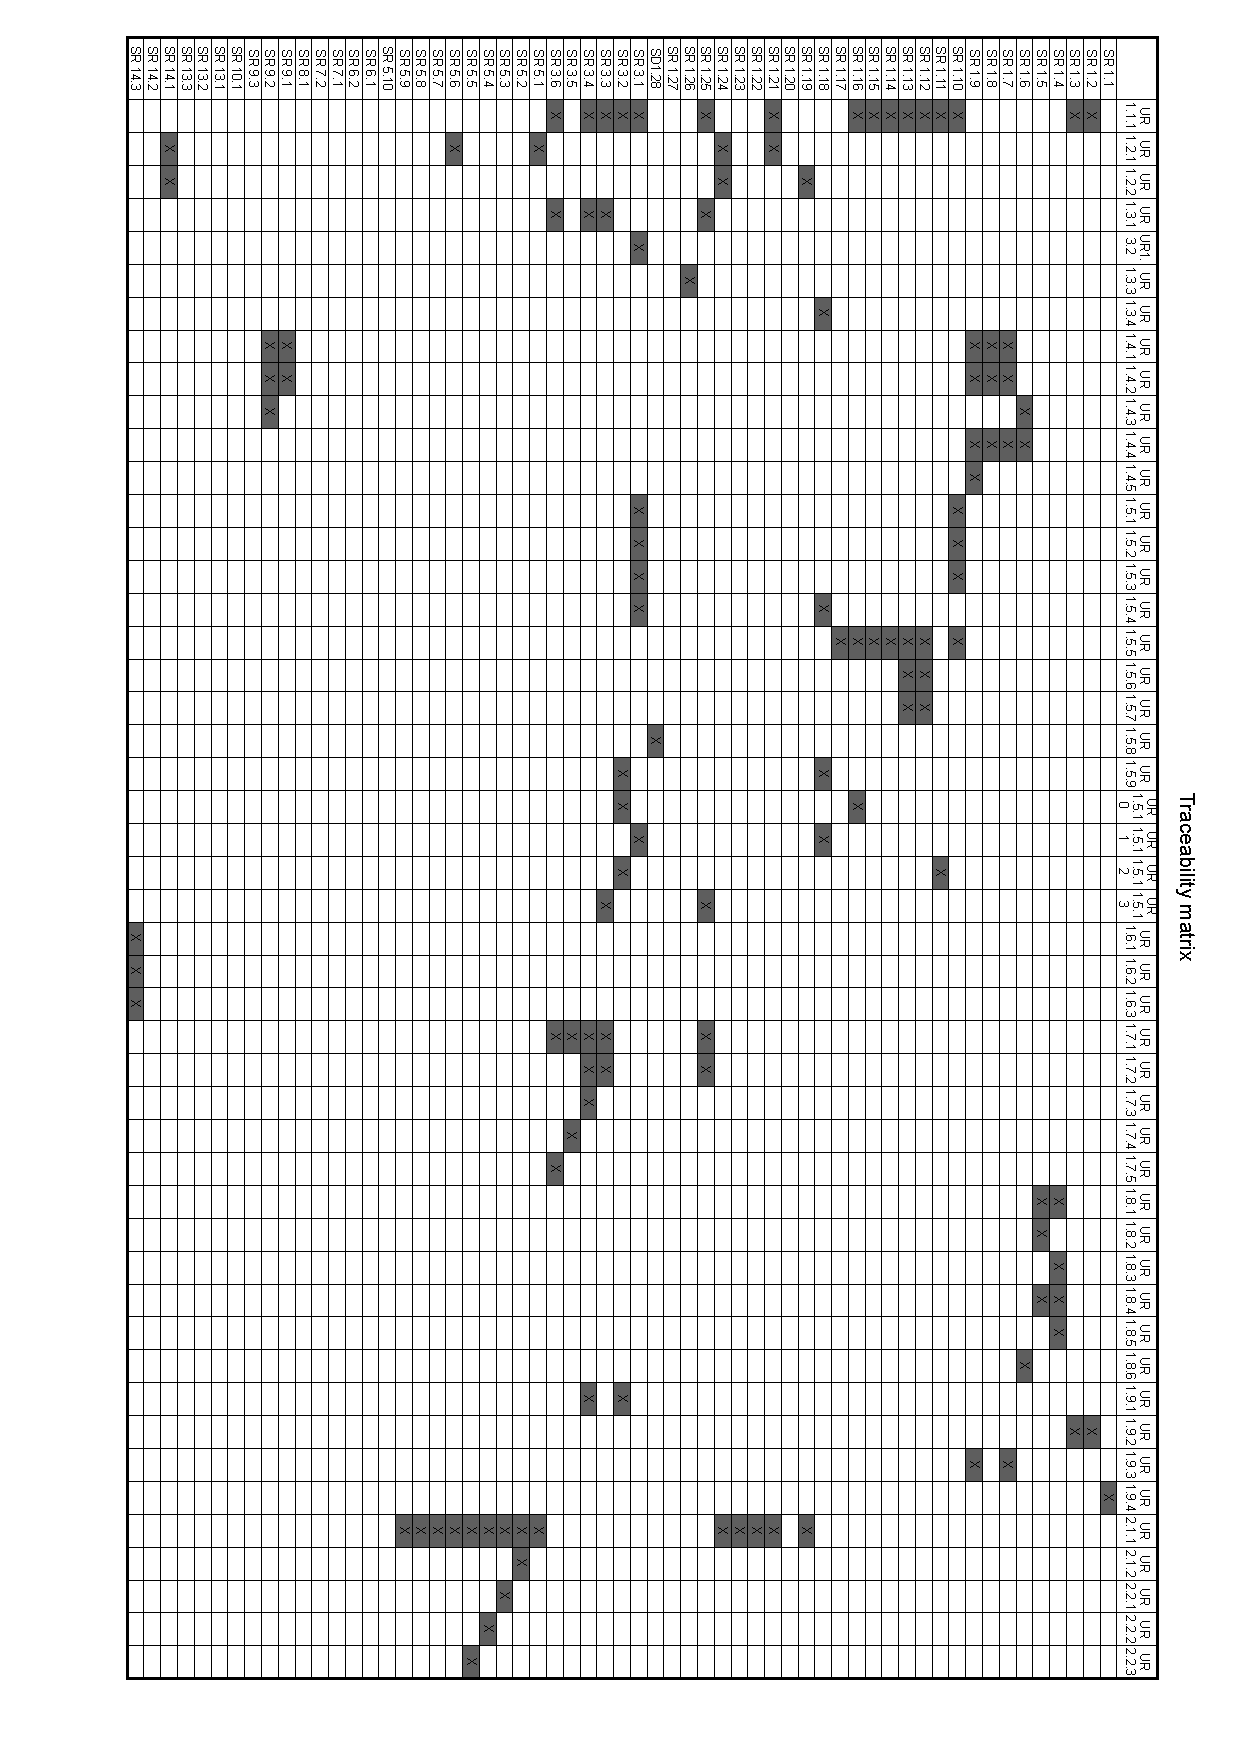
\includepdf{graphics/tracability-matrix.pdf} % Or wherever you'll choose to put it
\end{document}

